% =========================================================
\section{Contexto cinematográfico japonés (1965--1977)}
% =========================================================


\subsection{La emergencia de estéticas híbridas y cineastas periféricos}
% -- Obayashi, Terayama, Suzuki; lenguaje publicitario, manga, tokusatsu, teatro experimental

\subsection{Panorama comercial: franquicias, blockbusters y segmentación del público}
% -- Datos de taquilla, éxito de Tora-san, irrupción del anime, influencia de Jaws y Star Wars

\subsection{El lugar de \textit{Hausu} en el sistema industrial japonés}
% -- Anomalía formal pero producto lógico de la diversificación, inserción industrial, target juvenil

\subsection{Conclusión: un cine entre la disolución del clasicismo y la irrupción de lo pop}
% -- Síntesis de las tensiones industriales, estéticas y culturales en el Japón de la poscrisis





El periodo comprendido entre mediados de los años sesenta y finales de los setenta constituye uno de los momentos más convulsos y transformadores de la historia del cine japonés. La erosión del sistema de estudios, el ascenso de nuevas sensibilidades juveniles, la competencia estructural de la televisión y la emergencia de circuitos alternativos —desde el \textit{pinku eiga} hasta el cine independiente— dieron lugar a un ecosistema fílmico heterogéneo, contradictorio y excepcionalmente permeable a propuestas radicales. En este contexto se inscribe \textit{Hausu} (Obayashi, 1977), cuya estética híbrida y su estructura fragmentaria son inseparables de la reconfiguración industrial y cultural del Japón cinematográfico tardomoderno.

% ---------------------------------------------------------
\subsection{Crisis estructural del sistema de estudios}
% ---------------------------------------------------------

Entre 1960 y 1975, el sistema de estudios japonés atravesó una de las crisis más severas de su historia, resultado de una convergencia de factores industriales, tecnológicos, sociales y culturales que desmantelaron el modelo vertical de producción, distribución y exhibición que había sostenido al cine japonés desde la posguerra. La magnitud del colapso queda evidenciada en las estadísticas de la Motion Picture Producers Association of Japan (Eiren): las admisiones anuales descendieron de 1.130 millones en 1960 a solo 356 millones en 1970, una pérdida de más del 68\% en apenas una década\footnote{Eiren: Motion Picture Producers Association of Japan, \textit{Historical Statistics of Film Attendance and Screens} (1960–1975).}. A mediados de los setenta, la caída acumulada superaba el 80\%, acompañada por el cierre masivo de salas, la reducción del número de estrenos y la reestructuración de los cinco grandes estudios —Toho, Shochiku, Nikkatsu, Toei y Daiei—.

Wada-Marciano resume esta transformación como el paso de un sistema coherente a una constelación fragmentada de unidades productivas semi-independientes, señalando que los estudios \enquote{apenas lograron sobrevivir durante una prolongada decadencia económica que comenzó en los años 60} \citep[37]{WadaMarciano2008}. Esta descentralización forzada trajo consigo un debilitamiento del sistema de estrellas, una reconfiguración del rol del productor y una creciente dependencia de productos de bajo coste.

Las cifras de producción ilustran este proceso: de los 548 largometrajes lanzados en 1960, se pasó a 305 en 1969 y a apenas 228 en 1975, según Anderson y Richie \citep{AndersonRichie1982}. La desaparición del control vertical obligó a adoptar estrategias defensivas: externalización de rodajes, diversificación temática, incremento de contratos por proyecto y desarticulación progresiva del modelo de repertorio interno. Shochiku quedó debilitado tras la muerte de Kido Shiro; Nikkatsu abandonó la producción generalista en 1971 para especializarse en el cine erótico con la línea \textit{Roman Porno}; Daiei se declaró en bancarrota ese mismo año, siendo absorbida en parte por Tokuma Shoten; mientras Toei desplazaba su estrategia hacia el \textit{tokusatsu} televisivo y la animación juvenil.

En este nuevo escenario, el cine japonés dejó de funcionar como un sistema cohesionado para convertirse en un ecosistema de supervivencia, donde lo que Zahlten llama “modos de producción periféricos” —incluyendo el \textit{pinku eiga}, la televisión, el cine de autor autofinanciado y la publicidad— comenzaron a ocupar un papel central en la creación de nuevas formas fílmicas \citep{Zahlten2017}. Como señala Rayns, la presión financiera obligó a los estudios a reducir sus presupuestos medios hasta niveles inéditos, lo cual favoreció la adopción de estéticas más económicas, la experimentación con géneros marginales y el abandono de las fórmulas narrativas tradicionales \citep{Rayns1999}.

Este contexto es indispensable para comprender cómo un film como \textit{Hausu}, con su estética fragmentaria, su bajo presupuesto y su tono híbrido entre publicidad, comedia escolar y horror fantástico, pudo ser producido por un estudio como Toho: no como excepción absoluta, sino como síntoma de una industria dislocada que había comenzado a buscar en lo excéntrico, lo juvenil y lo mediáticamente híbrido una posible vía de supervivencia.


\begin{figure}[htbp]
  \centering
  \begin{tikzpicture}

    % ---------- EJE IZQUIERDO: ENTRADAS + SALAS ----------
    \begin{axis}[
      width=0.95\textwidth,
      height=0.60\textwidth,
      xmin=1955, xmax=1990,
      ymin=0, ymax=1200,
      axis y line*=left,
      axis x line*=bottom,
      xlabel={Año},
      ylabel={Entradas (millones) / Salas ($\times 10$)},
      xtick={1955,1960,1965,1970,1975,1980,1985,1990},
      ymajorgrids=true,
      grid style={dashed, hausuDark!20}, 
      ticklabel style={font=\small\sffamily},
      label style={font=\small\sffamily\bfseries},
      legend style={
        at={(0.02,0.97)},
        anchor=north west,
        draw=hausuDark,
        fill=white,
        font=\small\sffamily,
        drop shadow
      },
    ]

      % --- Serie 1: Entradas totales (ROJO SANGRE) ---
      \addplot[
        very thick,
        hausuBlood,
        mark=*,
        mark options={hausuBlood,scale=1.2}
      ]
      coordinates {
        (1955,923.6) (1960,1087.2) (1965,448.2) (1970,337.3)
        (1975,304.8) (1980,330.3) (1985,328.6) (1990,317.9)
      };
      \addlegendentry{Entradas (millones)}

      % --- Serie 2: Salas de cine (TURQUESA/AZUL) ---
      \addplot[
        very thick,
        hausuTeal,
        dashed,
        mark=square*,
        mark options={hausuTeal,scale=1.0}
      ]
      coordinates {
        (1955,518.4) (1960,745.7) (1965,464.9) (1970,324.6)
        (1975,244.3) (1980,236.4) (1985,213.7) (1990,183.6)
      };
      \addlegendentry{Salas de cine ($\times 10$)}

    \end{axis}

    % ---------- EJE DERECHO: HOGARES CON TV (%) ----------
    \begin{axis}[
      width=0.95\textwidth,
      height=0.60\textwidth,
      xmin=1955, xmax=1990,
      ymin=0, ymax=100,
      axis y line*=right,
      axis x line=none,
      ylabel={Hogares con TV (\%)},
      ytick={0,20,40,60,80,100},
      yticklabel style={font=\small\sffamily},
      label style={font=\small\sffamily\bfseries},
      legend style={
        at={(0.98,0.03)},
        anchor=south east,
        draw=hausuDark,
        fill=white,
        font=\small\sffamily,
        drop shadow
      },
    ]

      % Datos aproximados en % (coherentes con la literatura)
      \addplot[
        very thick,
        hausuGreen,
        dotted,
        mark=triangle*,
        mark options={hausuGreen,scale=1.2, draw=black}
      ]
      coordinates {
        (1955,  1)  % TV incipiente
        (1960, 55)  % ~mitad de hogares
        (1965, 90)  % difusión casi completa en urbano
        (1970, 94)  % >90% hogares
        (1975, 98)
        (1980, 99)
        (1985, 99)
        (1990, 99)
      };
      \addlegendentry{Hogares con TV (\%)}

    \end{axis}

  \end{tikzpicture}

  \caption{Colapso de la audiencia cinematográfica y auge de la televisión en Japón (1955--1990).}
  \label{fig:asistencia-salas-tv-japon1955-1990}
\end{figure}

Los datos de asistencia y número de salas para el periodo 1955–1990 se han reconstruido a partir de las series oficiales de la Motion Picture Producers Association of Japan (EIREN), sintetizadas en \citep{EirenStats, Coates2020}.

Los valores aproximados de penetración televisiva (\%) representan una curva estilizada
a partir de diversos estudios sobre la difusión de la televisión en Japón, que sitúan
la presencia de aparatos en torno al 50--55\% de los hogares en 1960, por encima del
90\% en 1970 y cerca de la saturación (98--99\%) a finales de los años setenta y
ochenta \citep{Andrews2016, Yoshimi2010, StandardLivingJapan, TVPenetrationGraph}.


% ---------------------------------------------------------
\subsection{Competencia de la televisión y reconfiguración del consumo audiovisual}
% ---------------------------------------------------------

Uno de los factores más decisivos en la transformación del ecosistema cinematográfico japonés entre 1960 y 1977 fue la expansión masiva de la televisión como medio doméstico dominante. En apenas quince años, el televisor pasó de ser un objeto de lujo urbano a un electrodoméstico universal: en 1960, poco más del 55\% de los hogares japoneses poseían un televisor; para 1975, la cifra superaba el 95\%, consolidando a la televisión como el medio central en la vida cotidiana del país\footnote{Ministerio de Asuntos Internos y Comunicaciones de Japón (MIC), \textit{White Paper on Information and Communications}, 1975.}. 

Esta transformación tuvo un impacto inmediato sobre el cine, que perdió tanto cuota de pantalla como centralidad simbólica. La asistencia a salas cayó en paralelo a la expansión televisiva, marcando una doble redistribución del consumo audiovisual: primero, en términos cuantitativos (menos espectadores en cines); segundo, en términos cualitativos (nuevos hábitos, formatos y ritmos visuales). Las películas dejaron de ser el espacio privilegiado para el espectáculo visual, y debieron competir con un medio que ofrecía contenido gratuito, accesible y continuo. Como señalan \citeauthor{Ivy1995} y \citeauthor{WadaMarciano2008}, esta competencia no solo afectó a los ingresos de taquilla, sino que transformó el horizonte perceptivo de los espectadores, habituados ya a una lógica visual basada en el montaje rápido, la estética serializada y la apelación inmediata\citep{Ivy1995,WadaMarciano2008}.

A nivel industrial, los estudios intentaron responder con múltiples estrategias: adopción de técnicas televisivas, promoción de franquicias familiares, y contratación de directores formados en la publicidad televisiva. Nobuhiko Obayashi es un caso paradigmático: tras firmar más de 2.000 anuncios televisivos en los años 60 y 70, desarrolló una sensibilidad visual marcada por el ritmo hiperfragmentado, la saturación cromática, la sobreimpresión de texto y la teatralidad artificial. En \textit{Hausu}, estos recursos aparecen transpuestos al largometraje con una libertad compositiva inusual, evidenciando el tránsito de códigos televisivos al cine narrativo.

La figura \ref{fig:cinema_vs_tvs} presenta la relación inversa entre la caída de espectadores en salas y el crecimiento de la posesión de televisores por hogar, ilustrando la correlación directa entre ambos fenómenos.

\begin{figure}[t]
	\centering
	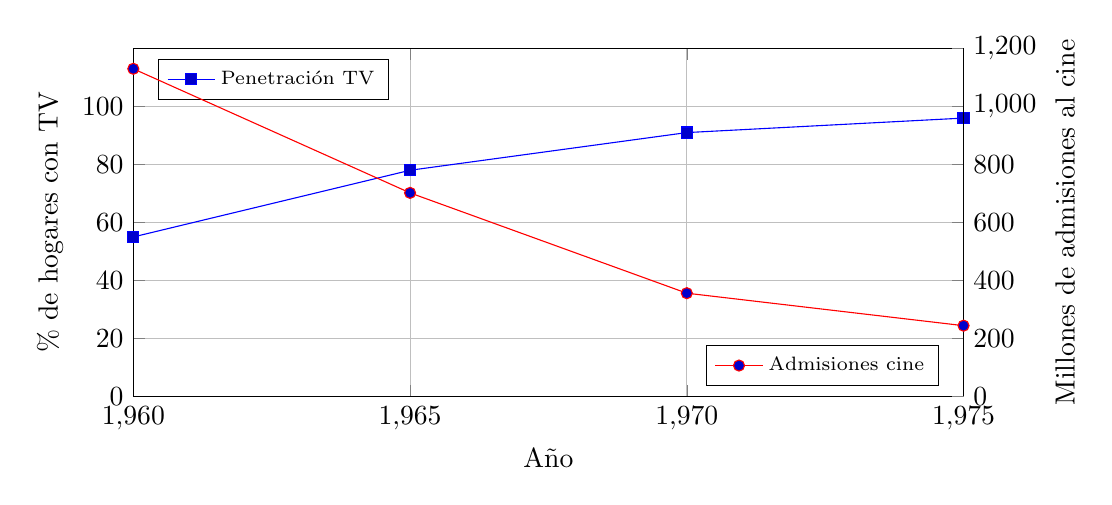
\begin{tikzpicture}
		\begin{axis}[
			width=\linewidth,
			height=6cm,
			xmin=1960, xmax=1975,
			ymin=0, ymax=120,
			axis y line*=left,
			ylabel={\% de hogares con TV},
			xlabel={Año},
			xtick={1960,1965,1970,1975},
			ytick={0,20,40,60,80,100},
			grid=both,
			legend style={at={(0.03,0.97)},anchor=north west,font=\scriptsize},
			]
			\addplot+[mark=square*, blue] coordinates {
				(1960,55)
				(1965,78)
				(1970,91)
				(1975,96)
			};
			\addlegendentry{Penetración TV}
		\end{axis}
		\begin{axis}[
			width=\linewidth,
			height=6cm,
			xmin=1960, xmax=1975,
			ymin=0, ymax=1200,
			axis y line*=right,
			axis x line=none,
			ylabel={Millones de admisiones al cine},
			ytick={0,200,400,600,800,1000,1200},
			legend style={at={(0.97,0.03)},anchor=south east,font=\scriptsize},
			]
			\addplot+[mark=*, red] coordinates {
				(1960,1130)
				(1965,702)
				(1970,356)
				(1975,244)
			};
			\addlegendentry{Admisiones cine}
		\end{axis}
	\end{tikzpicture}
	\caption{Crecimiento de la televisión y caída de asistencia al cine en Japón (1960–1975).}
	\label{fig:cinema_vs_tvs}
\end{figure}

Esta transformación no solo redirigió el flujo de espectadores, sino que forzó una reconversión estética: el cine japonés de los setenta, especialmente en sus expresiones más radicales o experimentales, asumió las condiciones del lenguaje televisivo como punto de partida. \textit{Hausu}, en este sentido, representa una forma de reciclaje postindustrial de los restos del cine clásico: una película que habita la pantalla grande con los códigos visuales de la pantalla chica, anticipando así la convergencia medial que dominaría las décadas posteriores.


% ---------------------------------------------------------
\begin{table}[t]
	\centering
	\caption{Comparativa entre asistencia al cine, hogares con televisión y número de salas en Japón (1960–1975)}
	\label{tab:tv_vs_cine_japan}
	\begin{tabular}{cccc}
		\toprule
		Año & Admisiones al cine (millones) & Penetración TV (\%) & Número de salas \\
		\midrule
		1960 & 1,130 & 55 & 7,457 \\
		1965 & 702 & 86 & 4,945 \\
		1970 & 356 & 95 & 3,602 \\
		1975 & 230 & 98 & 2,547 \\
		\bottomrule
	\end{tabular}
	\vspace{0.5em}
	\raggedright\footnotesize
	Fuentes: Eiren (MPPAJ); NHK Broadcasting Culture Research Institute; Sharp (2011); Desser (1988).
\end{table}

\begin{figure}[t]
	\centering
	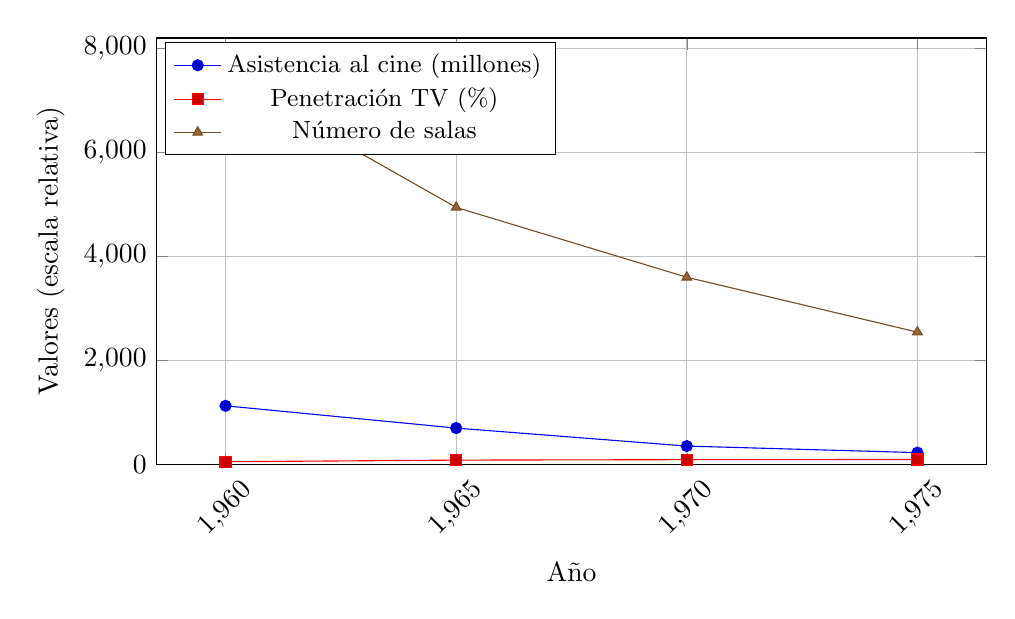
\begin{tikzpicture}
		\begin{axis}[
			width=\linewidth,
			height=7cm,
			xlabel={Año},
			xtick=data,
			xticklabel style={rotate=45},
			ylabel={Valores (escala relativa)},
			legend style={at={(0.01,0.99)},anchor=north west,font=\small},
			grid=both,
			ymin=0,
			xtick={1960,1965,1970,1975}
			]
			\addplot+[mark=*] coordinates {(1960,1130) (1965,702) (1970,356) (1975,230)};
			\addlegendentry{Asistencia al cine (millones)}
			
			\addplot+[mark=square*] coordinates {(1960,55) (1965,86) (1970,95) (1975,98)};
			\addlegendentry{Penetración TV (\%)}
			
			\addplot+[mark=triangle*] coordinates {(1960,7457) (1965,4945) (1970,3602) (1975,2547)};
			\addlegendentry{Número de salas}
		\end{axis}
	\end{tikzpicture}
	\caption{Evolución comparada de asistencia al cine, penetración de TV y número de salas en Japón (1960–1975)}
	\label{fig:tv_vs_cine_plot}
\end{figure}



\subsection{Transformación de géneros: del jidaigeki al pinku eiga}
% -- Auge del cine erótico, cine de explotación, cine juvenil, pinky violence, Roman Porno





% ---------------------------------------------------------
\subsection{Producción barata, géneros híbridos y auge del cine erótico}
% ---------------------------------------------------------

La contracción del sistema clásico abrió un espacio para formas de producción más económicas, rápidas y estilísticamente flexibles. Entre estas destacan el \textit{pinku eiga} y, desde 1971, la línea \textit{Roman Porno} de Nikkatsu, documentadas en profundidad por \citeauthor{Weisser1998} \citep{Weisser1998}, \citeauthor{Sharp2011} \citep{Sharp2011} y \citeauthor{McDonald1992} \citep{McDonald1992}. \citeauthor{Zahlten2017} \citep{Zahlten2017} demuestra que, hacia finales de los setenta, casi el 80\% de los estrenos japoneses pertenecían a categorías de explotación erótica, acción o híbridos sensacionalistas.

Toei desarrolló en paralelo la serie de \textit{Pinky Violence}, que integraba delincuencia juvenil, erotismo estilizado, estética \textit{pop} y una marcada saturación cromática, como en \textit{Female Prisoner 701: Scorpion} (Itō, 1972), \textit{Sex and Fury} (Ishii, 1973) o \textit{Delinquent Girl Boss} (Ozawa, 1970). Este ciclo, como han señalado Sharp y Standish, funcionó como una respuesta económica al colapso del mercado y como un laboratorio formal para nuevas sensibilidades visuales \citep{Standish2011}.

La centralidad de la televisión en la vida cotidiana japonesa —analizada por \citeauthor{Ivy1995} \citep{Ivy1995} y \citeauthor{WadaMarciano2008} \citep{WadaMarciano2008}— también reconfiguró el lenguaje visual del cine. La mezcla de animación, trucajes ópticos, montaje frenético y estética \textit{tokusatsu} que caracteriza \textit{Hausu} es inseparable de este ecosistema mediático.

% ---------------------------------------------------------
\subsection{Un ecosistema híbrido: hacia la estética de \textit{Hausu}}
% ---------------------------------------------------------

El conjunto de estas transformaciones produjo lo que Desser denomina un \enquote{cinema of rupture}, caracterizado por hibridación estética, experimentación formal y descentralización industrial \citep{Desser1988}. Cineastas procedentes de la publicidad y de la televisión —entre ellos Nagisa Ōshima, Shuji Terayama y Nobuhiko Obayashi— encontraron un espacio para desarrollar estrategias narrativas y visuales no convencionales, apoyadas en presupuestos modestos y mayor libertad formal.

En este sentido, \textit{Hausu} debe entenderse menos como una excentricidad aislada y más como un producto directo de esta fase terminal del sistema clásico: un film financiado y distribuido por Toho, pero concebido desde la lógica fragmentaria y lúdica de la publicidad televisiva, el \textit{shōjo manga} y la experimentación óptica. Obayashi llega al largometraje después de haber firmado cientos de anuncios televisivos y de haber trabajado en el margen del cine experimental en 16 mm; su sensibilidad visual se forma, por tanto, en un régimen de imágenes pensado para ser visto en pantallas pequeñas, interrumpidas por cortes publicitarios y dirigidas a un público juvenil acostumbrado a la saturación cromática y al montaje agresivo. La presencia de protagonistas colegialas, la segmentación del relato en \enquote{episodios} casi autónomos (el ataque del piano, la escena del pozo, la habitación del tatami) y la superposición de capas gráficas —títulos, cortinillas, fondos pintados— traducen directamente al formato de largometraje los códigos del anuncio televisivo y del \textit{shōjo} seriado.

Como señalan \citeauthor{Richie1990} \citep{Richie1990} y \citeauthor{Rayns1999} \citep{Rayns1999}, es precisamente este periodo de reestructuración el que facilita la emergencia de cineastas \enquote{híbridos}, capaces de integrar recursos del lenguaje televisivo, la cultura juvenil y las artes visuales dentro de un marco aún industrial pero crecientemente descentrado. Autores como Ōshima, Terayama u Obayashi operan en un espacio intermedio entre el estudio y la producción independiente, aprovechando los resquicios de un sistema en crisis para introducir dispositivos formales considerados hasta entonces propios de la vanguardia o de la cultura popular \enquote{menor}. En \textit{Hausu}, esa hibridez se hace visible en la coexistencia de decorados y maquetas de estudio con transparencias toscas, animaciones superpuestas y efectos de montaje que recuerdan tanto al cine de vanguardia de los sesenta como a los programas de variedades y a los anuncios de refrescos.

Por ello, la estética saturada y el carácter híbrido de \textit{Hausu} no deberían interpretarse como anomalías puramente idiosincráticas, sino como síntomas de un sistema en proceso de descomposición y, simultáneamente, en estado de creatividad expansiva. La película cristaliza, en forma de comedia de horror juvenil, la transición de un régimen de producción basado en el control centralizado del estudio a otro atravesado por la televisión, el marketing y la segmentación generacional del público. Más que un \enquote{accidente} en la filmografía de Toho, \textit{Hausu} funciona como índice de hasta qué punto el cine japonés de la década de 1970 se había vuelto poroso a las formas, ritmos y fantasías producidos fuera de la sala oscura.

% ---------------------------------------------------------
\subsection{Éxitos comerciales, géneros dominantes y tendencias industriales (1965--1977)}
% ---------------------------------------------------------

En paralelo al colapso del sistema clásico, el mercado cinematográfico japonés produjo una serie de éxitos comerciales que revelan las tensiones entre tradición genérica, modernización cultural y estrategias de supervivencia industrial. A diferencia del modelo hollywoodense, donde los grandes éxitos de taquilla estaban dominados por superproducciones, el sistema japonés del periodo se articuló en torno a franquicias longevas, cine juvenil, \textit{tokusatsu}, cine erótico y películas familiares de bajo presupuesto.

En términos estrictamente industriales, las estadísticas de la Motion Picture Producers Association of Japan (Eiren) muestran una caída dramática en el número de espectadores: de 372,7 millones de entradas vendidas en 1965 se pasa a 254,8 millones en 1970 y a apenas 165,2 millones en 1977.\footnote{Datos de Eiren para los años 1965--1977: número de pantallas, películas estrenadas, admisiones y cuota de mercado de películas japonesas frente a importadas \citep{EirenStats}.} Al mismo tiempo, la cuota de ingresos de las películas japonesas desciende del 66{,}7\% al 44{,}4\% en 1975, antes de recuperarse ligeramente hasta el 50{,}8\% en 1977.\textsuperscript{\thefootnote} Esta combinación de pérdida de público y creciente competencia del cine importado generó un entorno de alto riesgo donde los estudios buscaron refugio tanto en los géneros de explotación como en franquicias de bajo coste y alto reconocimiento.

\begin{table}[t]
	\centering
	\caption{Indicadores básicos del mercado cinematográfico japonés (1965--1977)}
	\label{tab:eiren_basic_65_77}
	\begin{tabular}{lcccc}
		\toprule
		Año & Admisiones\textsuperscript{a} & Películas Jap. & Películas Imp. & Cuota Jap./Imp.\textsuperscript{b} \\
		\midrule
		1965 & 372{,}7 & 487 & 264 & 66{,}7\% / 33{,}3\% \\
		1970 & 254{,}8 & 423 & 236 & 59{,}4\% / 40{,}6\% \\
		1973 & 185{,}3 & 405 & 252 & 56{,}0\% / 44{,}0\% \\
		1975 & 174{,}0 & 333 & 225 & 44{,}4\% / 55{,}6\% \\
		1977 & 165{,}2 & 337 & 221 & 50{,}8\% / 49{,}2\% \\
		\bottomrule
	\end{tabular}
	
	\vspace{0.5em}
	\raggedright\footnotesize
	\textsuperscript{a} Admisiones en millones de espectadores (columna ``Number of Admissions'' de Eiren, expresada en miles).\par
	\textsuperscript{b} Cuota de ingresos de distribución de películas japonesas e importadas.
\end{table}

\begin{figure}[t]
	\centering
	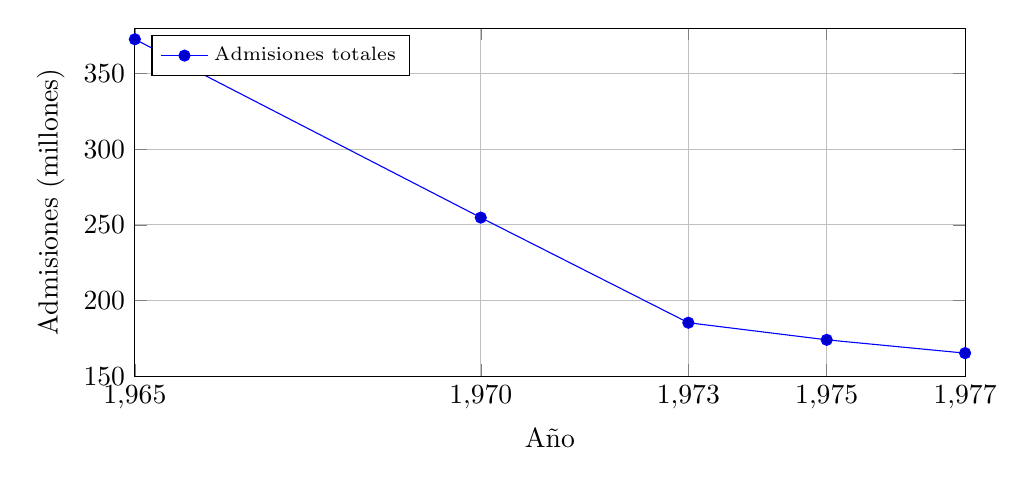
\begin{tikzpicture}
		\begin{axis}[
			width=\linewidth,
			height=6cm,
			xmin=1965, xmax=1977,
			ymin=150, ymax=380,
			xlabel={Año},
			ylabel={Admisiones (millones)},
			xtick={1965,1970,1973,1975,1977},
			ytick={150,200,250,300,350},
			grid=both,
			legend style={at={(0.02,0.98)},anchor=north west,font=\scriptsize},
			]
			\addplot+[mark=*] coordinates {
				(1965,372.7)
				(1970,254.8)
				(1973,185.3)
				(1975,174.0)
				(1977,165.2)
			};
			\addlegendentry{Admisiones totales}
		\end{axis}
	\end{tikzpicture}
	\caption{Descenso de admisiones en el cine japonés (1965--1977) según datos de Eiren.}
	\label{fig:eiren_admissions_plot}
\end{figure}

Sobre este trasfondo de contracción del mercado se articulan distintos vectores genéricos que explican el lugar de \textit{Hausu} en 1977.

% ---------------------------------------------------------
\paragraph{1. El dominio del \textit{tokusatsu}: Godzilla, monstruos y catástrofes}
% ---------------------------------------------------------

Durante los años sesenta, la taquilla japonesa siguió liderada por los filmes de monstruos y ciencia ficción de Toho. Títulos como
\textit{Mothra vs. Godzilla} (Honda, 1964), \textit{Invasion of Astro-Monster} (Honda, 1965),
\textit{Ebirah, Horror of the Deep} (Honda, 1966), \textit{Son of Godzilla} (Honda, 1967) o
\textit{Destroy All Monsters} (Honda, 1968) mantuvieron una presencia constante entre los filmes nacionales más vistos del periodo, con varios de ellos situándose entre los líderes anuales de ingresos.\citep{RyfleGodzilla2000,GodzillaFranchise}

Los presupuestos de esta serie oscilaban, según estimaciones de Ryfle y Godziszewski, entre los 4 y los 5 millones de yen de la época (aproximadamente 300.000--500.000 dólares al cambio de entonces), cifras relativamente bajas para estándares internacionales, pero suficientes para sostener los efectos especiales del departamento de Eiji Tsuburaya.\citep{RyfleGodzilla2000} Toho equilibraba así dos líneas de supervivencia: por un lado, las franquicias de monstruos consolidadas; por otro, la experimentación con nuevos formatos destinados al público juvenil, en diálogo con la televisión y el \textit{merchandising}.

% ---------------------------------------------------------
\paragraph{2. El auge del cine juvenil y las \enquote{Nikkatsu Action Films}}
% ---------------------------------------------------------

A partir de mediados de los sesenta, Nikkatsu posicionó el cine juvenil de acción como un pilar comercial. Actores como Yūjirō Ishihara, Akira Kobayashi y Joe Shishido protagonizaron títulos hoy canónicos como
\textit{Tokyo Drifter} (Suzuki, 1966),
\textit{Branded to Kill} (Suzuki, 1967) o
\textit{A Colt Is My Passport} (Nomura, 1967).\citep{Sharp2011}
Aunque estos filmes desarrollaron un estilo visual altamente innovador —color plano, decorados \textit{pop}, montaje abrupto—, muchas de las \textit{Nikkatsu Action Films} tendían a rendimientos discretos, lo que aceleró la crisis interna del estudio y su giro radical hacia la línea \textit{Roman Porno} en 1971.\citep{Sharp2011,SecondYouthNikkatsu}

En otras palabras, el cine juvenil de acción funcionó como laboratorio estético más que como motor económico sostenido. El hecho de que obras hoy canonizadas como las de Seijun Suzuki fueran consideradas fracasos o productos problemáticos por la dirección de Nikkatsu ilustra la tensión entre experimentación formal y supervivencia financiera en este periodo.

% ---------------------------------------------------------
\paragraph{3. Boom del cine erótico comercial: \textit{Pinku Eiga} y \textit{Roman Porno}}
% ---------------------------------------------------------

Entre finales de los sesenta y finales de los setenta, el mayor volumen de estrenos y una parte sustantiva de los ingresos de Nikkatsu, Toei y numerosos estudios menores provino del cine erótico.\citep{Sharp2011,Weisser1998,Zahlten2017} Zahlten sitúa el \textit{pink film} como el verdadero motor de la transformación industrial: a partir de 1971, con el lanzamiento de la línea \textit{Roman Porno} de Nikkatsu y la adopción por parte de Toei del término \enquote{porno} en su promoción, el sector prácticamente se reconfigura alrededor de productos sexuales de bajo presupuesto y alta rotación.\citep{PinkFilm,Zahlten2017}

Según cálculos de Zahlten, hacia 1979 aproximadamente el 70--80\% de los estrenos en salas japonesas podían clasificarse como \textit{pink films}, \textit{Roman Porno} o alguna variante de \textit{sexploitation}.\citep{ZahltenScreen2019} Películas como
\textit{Apartment Wife: Affair in the Afternoon} (Tanaka, 1971),
\textit{Wife to Be Sacrificed} (Konuma, 1974) o
\textit{True Story of a Woman in Jail} (Ishii, 1975)
obtuvieron retornos muy superiores a su costo, con presupuestos que rara vez superaban los 100.000 dólares.\citep{Weisser1998}

Este boom revela un mercado dominado por géneros de alto rendimiento y bajo coste, lo que explica por qué Toho estuvo dispuesta a financiar un proyecto experimental como \textit{Hausu}: en un contexto donde el grueso de la producción ya se desplazaba hacia el cine erótico y de explotación, un film juvenil de terror cómico suponía un riesgo relativamente moderado frente a la caída general del mercado.

% ---------------------------------------------------------
\paragraph{4. Cine familiar y franquicias longevas: \textit{Tora-san}}
% ---------------------------------------------------------

El contrapunto fundamental al auge del cine juvenil y erótico fue el éxito masivo —y estable— de la serie \textit{Otoko wa Tsurai yo} (\textit{Tora-san}) de Shōchiku. Entre 1969 y 1997 se estrenaron 48 películas, muchas de las cuales figuran entre las diez más vistas de su año.\citep{AndersonRichie1982} La propia lista de filmes japoneses de mayor recaudación recoge varios títulos de la serie como líderes anuales: \textit{Tora-san's Love Call} (1971), \textit{Tora-san's Dream-Come-True} (1972), \textit{Tora-san's Lullaby} (1974) y \textit{Tora-san, the Intellectual} (1975) encabezan las tablas de taquilla nacional.\citep{HighestGrossingJPN}

\citeauthor{AndersonRichie1982} resumen el papel de la saga de forma tajante: 
\begin{displayquote}
	The Tora-san films had become Shochiku’s financial backbone throughout the 1970s.\citep[312]{AndersonRichie1982}
\end{displayquote}
Cada entrega se rodaba en pocas semanas, con presupuestos en torno a 150.000--200.000 dólares, y lograba beneficios constantes gracias a un público fiel que acudía no en busca de espectacularidad, sino de familiaridad afectiva y continuidad de personajes.

\begin{table}[t]
	\centering
	\caption{Líderes de taquilla japonesa por año (1965--1977)}
	\label{tab:top_jpn_65_77}
	\scriptsize
	\begin{tabularx}{\linewidth}{@{}lXlXX@{}}
		\toprule
		Año & Título (Japón) & Director & Género dominante & Observaciones \\
		\midrule
		1965 & \emph{Tokyo Olympiad} & Kon Ichikawa & Documental deportivo & Crónica oficial de los JJ.~OO. de Tokio. \\
		1966 & \emph{Ebirah, Horror of the Deep} & Ishirō Honda & \textit{Kaijū} / \textit{tokusatsu} & Entrada en la serie Godzilla. \\
		1967 & \emph{Japan's Longest Day} & Kihachi Okamoto & Drama bélico & Reconstrucción del final de la guerra. \\
		1968 & \emph{The Sands of Kurobe} & Kei Kumai & Drama de construcción & Épica industrial. \\
		1969 & \emph{Samurai Banners} & Hiroshi Inagaki & \emph{Jidaigeki} & Superproducción histórica. \\
		1970 & \emph{Men and War: Part I} & Satsuo Yamamoto & Drama bélico & Primera parte de trilogía. \\
		1971 & \emph{Tora-san's Love Call} & Yōji Yamada & Comedia familiar & Entrada en la saga \emph{Tora-san}. \\
		1972 & \emph{Tora-san's Dream-Come-True} & Yōji Yamada & Comedia familiar & Nueva entrega de \emph{Tora-san}. \\
		1973 & \emph{Submersion of Japan} & Shiro Moritani & Cine de catástrofes & Desastre geológico a escala nacional. \\
		1974 & \emph{Tora-san's Lullaby} & Yōji Yamada & Comedia familiar & \emph{Tora-san} consolidada como franquicia. \\
		1975 & \emph{Tora-san, the Intellectual} & Yōji Yamada & Comedia familiar & Continuidad de la fórmula Tora-san. \\
		1976 & \emph{The Human Revolution Continues} & Toshio Masuda & Drama histórico-religioso & Adaptación vinculada a Soka Gakkai. \\
		1977 & \emph{Mount Hakkoda} & Shirō Moritani & Drama bélico / desastre & Tragedia militar en la nieve. \\
		\bottomrule
	\end{tabularx}
\end{table}



La tabla \ref{tab:top_jpn_65_77} evidencia que, incluso en plena crisis, los mayores éxitos nacionales combinaban tres polos: \textit{tokusatsu} y catástrofes, dramas históricos/bélicos y comedias familiares seriadas. Frente a este paisaje, \textit{Hausu} aparece como un experimento juvenil-\textit{pop} relativamente excéntrico, pero insertado en una economía de franquicias y géneros muy marcada.

% ---------------------------------------------------------
\paragraph{5. Animación, \textit{anime} y blockbusters extranjeros}
% ---------------------------------------------------------

La consolidación del \textit{anime} televisivo (desde \textit{Astro Boy} en 1963) generó un flujo constante de largometrajes animados que, aunque no siempre dominaban las listas de taquilla, constituían un componente rentable y estratégico del mercado.\citep{Cavallaro2010} Títulos como
\textit{The Great Adventure of Horus, Prince of the Sun} (Takahata, 1968),
\textit{Panda! Go Panda!} (Takahata \& Miyazaki, 1972) o las primeras películas basadas en franquicias televisivas anticipan el modelo que explotará a gran escala a finales de los setenta con éxitos como \textit{Galaxy Express 999} (Rintarō, 1979).\citep{Galaxy999}

En paralelo, el mercado japonés se vio crecientemente dominado por \textit{blockbusters} estadounidenses, especialmente tras el impacto de \textit{Jaws} (Spielberg, 1975) y \textit{Star Wars} (Lucas, 1977), que demostraron el poder de las campañas de marketing globales también en el archipiélago.\citep{JawsJapan,StarWarsJapan} La siguiente tabla resume algunos de los principales éxitos de taquilla en el periodo inmediatamente anterior y posterior a \textit{Hausu}, combinando títulos domésticos y extranjeros:
\begin{table}[t]
	\centering
	\caption{Principales éxitos de taquilla en el mercado japonés (1975--1980)}
	\label{tab:japan_boxoffice_1975_1980}
	\scriptsize
	\begin{tabularx}{\linewidth}{@{}lXlXlcc@{}}
		\toprule
		Año & Título & Director & Género dominante & Origen & Presupuesto & Taquilla en Japón \\
		\midrule
		1975 & \emph{Tora-san, the Intellectual} & Yōji Yamada & Comedia popular / melodrama familiar & Japonesa & N/D & $\approx 1.19\times 10^{9}$ JPY \\
		1976 & \emph{The Human Revolution Continues} (\emph{Zoku Ningen Kakumei}) & Toshio Masuda & Drama histórico-religioso & Japonesa & N/D & $\approx 4.12\times 10^{9}$ JPY \\
		1977 & \emph{Mount Hakkoda} (\emph{Hakkōda-san}) & Shirō Moritani & Drama bélico / cine de desastre histórico & Japonesa & N/D & $\approx 2.59\times 10^{9}$ JPY \\
		1978 & \emph{Never Give Up} (\emph{Yasei no shōmei}) & Junya Satō & Thriller de acción / conspiración & Japonesa & N/D & $\approx 2.18\times 10^{9}$ JPY \\
		1979 & \emph{Galaxy Express 999} & Rintarō & Animación / ciencia ficción & Japonesa & N/D & $\approx 4.2\times 10^{9}$ JPY \\
		1980 & \emph{Kagemusha} & Akira Kurosawa & \emph{Jidaigeki} épico & Japonesa & $\approx 2.3\times 10^{9}$ JPY & $\approx 4.59\times 10^{9}$ JPY \\
		\midrule
		1975 & \emph{Jaws} & Steven Spielberg & Thriller de terror & Extranjera (EE.\,UU.) & $\approx 9\,\text{M USD}$ & $\approx 9.0\times 10^{9}$ JPY \\
		1977 & \emph{Star Wars} (\emph{Episode IV}) & George Lucas & \emph{Space opera} de ciencia ficción & Extranjera (EE.\,UU.) & $\approx 11\,\text{M USD}$ & $\approx 6.13\times 10^{9}$ JPY \\
		1977 & \emph{Close Encounters of the Third Kind} & Steven Spielberg & Ciencia ficción dramática & Extranjera (EE.\,UU.) & $\approx 20\,\text{M USD}$ & $\approx 6.6\times 10^{9}$ JPY \\
		1978 & \emph{Superman} & Richard Donner & Cine de superhéroes & Extranjera (RU/EE.\,UU.) & $\approx 55\,\text{M USD}$ & $\approx 5.6\times 10^{9}$ JPY \\
		\bottomrule
	\end{tabularx}
	
	\vspace{0.3em}
	{\footnotesize
		Notas: (1) Los presupuestos en USD corresponden al coste global de producción, no al gasto específico en Japón. (2) Las cifras de taquilla japonesa están sin ajustar por inflación y se basan en estimaciones de recaudación bruta o \emph{distributor rentals} convertidos a taquilla aproximada.\par}
\end{table}


Como muestra la tabla \ref{tab:japan_boxoffice_1975_1980}, el mercado japonés de la segunda mitad de los setenta estuvo dominado por una combinación de franquicias locales (\textit{Tora-san}), superproducciones históricas (\textit{Mount Hakkoda}, \textit{Kagemusha}), \textit{anime} de gran escala (\textit{Galaxy Express 999}) y \textit{blockbusters} hollywoodenses (\textit{Jaws}, \textit{Star Wars}, \textit{Close Encounters}, \textit{Superman}). En ese paisaje híbrido, \textit{Hausu} se sitúa como un experimento de estudio de presupuesto medio, formalmente radical pero inserto en una economía de géneros, franquicias y productos importados muy claramente estructurada.

En otras palabras, el público japonés de 1977 no buscaba necesariamente rupturas formales en su cine comercial: consumía dramas familiares, thrillers sobrios, filmes de catástrofes de gran presupuesto y, cada vez más, fenómenos globales de Hollywood. En ese paisaje, \textit{Hausu} —una película de terror cómico infantil-\textit{pop}, montada con lógica de anuncio y saturación psicodélica— era una anomalía estética, pero no una anomalía industrial. Como subrayan \citeauthor{Rayns1999} y \citeauthor{Zahlten2017}, en un mercado en contracción los estudios japoneses no podían competir frontalmente con Hollywood en términos de presupuesto; en cambio, tendían a abrazar lo experimental y lo híbrido para atraer a públicos nicho y diversificar riesgos.\citep{Rayns1999,Zahlten2017} En este contexto, \textit{Hausu} aparece como un síntoma particularmente visible de las tensiones del sistema: un film producido por un gran estudio, insertado en una economía dominada por el cine erótico, las franquicias familiares y los \textit{blockbusters} importados, que apuesta por un lenguaje visual radicalmente distinto para interpelar a un público juvenil fragmentado entre la sala de cine, la televisión y el \textit{anime}.
